% =========================================================
% REVTeX 4.2 - APS sample look (apssamp-style) + VDM slots
% =========================================================
\documentclass[%
 reprint,                % <- use 'preprint' for 1-col manuscript; 'reprint' mimics journal
 superscriptaddress,     % author affiliations like sample
 %groupedaddress,        % (toggle options as needed)
 %unsortedaddress,
 %runinaddress,
 %frontmatterverbose,
 %preprintnumbers,
 %nofootinbib,
 %nobibnotes,
 %bibnotes,
 aps,                    % APS family
 prx,                    % prl/prx/pra/prb/prc/prd/pre etc.
 %longbibliography,      % (optional)
]{revtex4-2}

% ------------------- Packages (as in sample spirit) -------------------
\usepackage[T1]{fontenc}
\usepackage[utf8]{inputenc}
\usepackage{lmodern}
\usepackage{microtype}
\usepackage{graphicx}      % \includegraphics
\usepackage{dcolumn}       % decimal-aligned columns
\usepackage{bm}            % bold math
\usepackage{amsmath,amssymb}
\usepackage{hyperref}      % hyperlinks
\usepackage[nameinlink,capitalize]{cleveref} % clean refs (harmless w/ REVTeX)
\usepackage{siunitx}
\sisetup{detect-all}

% ------------------- Metadata -------------------
\begin{document}
\preprint{VDM-Results} % optional preprint mark

\title{Manuscript Title:\\ with Forced Linebreak} % sample shows forced linebreak via \\
\author{Justin K.\ Lietz}
\email{justin@neuroca.ai}
\affiliation{Neuroca, Inc.}
%\collaboration{MUSO Collaboration}\noaffiliation  % sample shows collaboration lines
%\author{Charlie Author}
%\affiliation{Second institution and/or address}
%\collaboration{CLEO Collaboration}\noaffiliation

\date{\today}

% ------------------- Abstract -------------------
\begin{abstract}
A concise summary of scope, method (standard term first; project label in parentheses),
primary gate(s) with thresholds, and where the evidence lives (figures/tables/artifacts).
\end{abstract}

\maketitle

% ====================== I. INTRODUCTION ======================
\section{Introduction}
State precisely what is and is not claimed. Give the evaluation question in one sentence.
Keep related work focused (2–4 citations) at the first skeptical touchpoints.

% ====================== II. BACKGROUND =======================
\section{Background}
\subsection{Scope and larger theory}
Situate within a standard framework (e.g., gradient flows/Onsager; metriplectic structure) and why it fits.

\subsection{Core equations used later}
List only the equations actually used (invariants, discretizations, error models) with symbol definitions and units.

\subsection{Map to gates}
Tie each property to the concrete metric/threshold tested in \cref{sec:results,sec:gates}.

% ====================== III. METHODS =========================
\section{Methods}
\subsection{Variables}
Independent/dependent variables, units and justified ranges; estimator and uncertainty.

\subsection{Equipment / Software}
Hardware, ROCm version, library versions, precision/modes.

\subsection{Procedure}
Steps sufficient for replication (third-person, past tense).

\subsection{Provenance}
\noindent\textbf{Commit:} \texttt{<commit-hash>}\quad
\textbf{Seed:} \texttt{<seed>}\quad
\textbf{Artifacts:} \texttt{<https://…/artifacts/>}

% ====================== IV. RESULTS ==========================
\section{Results}
\label{sec:results}
One claim per figure. Captions carry the numbers (slope, $R^2$, RMSE) and the paired CSV/JSON
filenames plus seed/commit.

\begin{figure}[t]
  \centering
  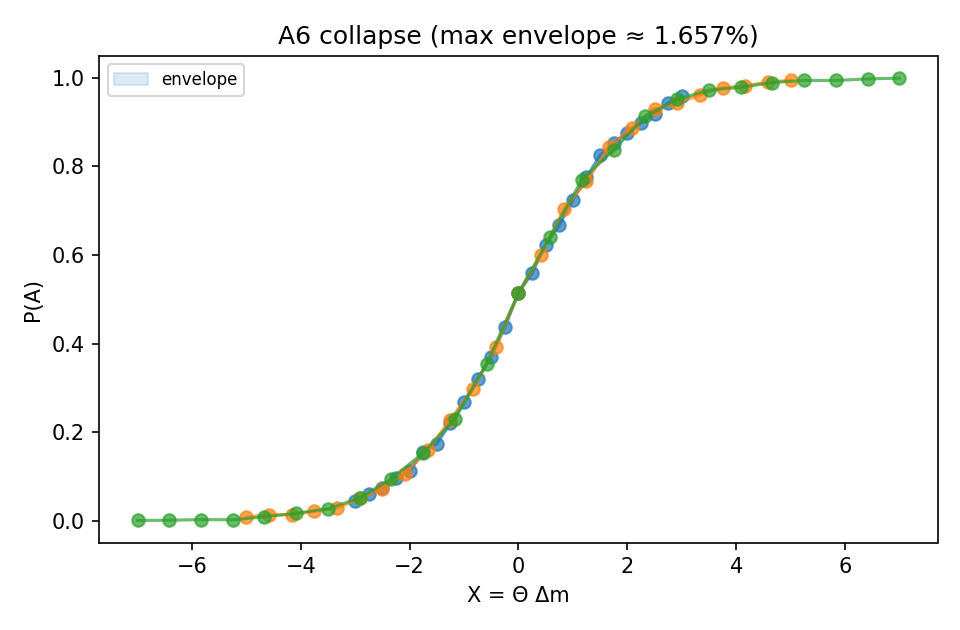
\includegraphics[width=\linewidth]{fig_1} % PDF/PNG preferred with pdfLaTeX
  \caption{Front-speed vs.\ theory; slope $0.98$, $R^2=0.995$.
  Paired artifacts: \texttt{front\_speed.csv}, \texttt{front\_speed.json};
  seed \texttt{<seed>}, commit \texttt{<commit>}.}
  \label{fig:frontspeed}
\end{figure}

\begin{table}[t]
  \caption{Summary metrics with uncertainties (sample uses \texttt{ruledtabular}).}
  \label{tab:summary}
  \begin{ruledtabular}
  \begin{tabular}{lccc}
    Metric & Mean & Std & $N$ \\
    \hline
    <metric A> & <..> & <..> & <..> \\
  \end{tabular}
  \end{ruledtabular}
\end{table}

% Wide figure/table examples (match sample layout in two-column reprint mode):
% \begin{figure*}[t]
%   \includegraphics[width=0.95\textwidth]{fig_2}
%   \caption{Wide figure spanning both columns (use figure*).}
%   \label{fig:wide}
% \end{figure*}

% \begin{table*}[t]
%   \caption{Wide table across both columns (use table*).}
%   \label{tab:wide}
%   \begin{ruledtabular}
%   \begin{tabular}{lccc}
%     ...
%   \end{tabular}
%   \end{ruledtabular}
% \end{table*}

% ====================== V. GATES & CONTRADICTIONS ============
\section{Gates and Contradiction Reports}
\label{sec:gates}
\noindent\textbf{Gate: Front-speed accuracy} (threshold: relative error $\le 5\%$).\\
Measured $3.2\%$ on $n=8$ seeds. \textbf{PASS}. Artifacts: \texttt{front\_speed.csv/json}.

\medskip
\noindent\textbf{Gate: Dispersion RMSE} (threshold: $\mathrm{RMSE}\le 2\times10^{-3}$).\\
Measured $2.4\times10^{-3}$. \textbf{FAIL}. See contradiction report \texttt{dispersion\_fail.json}.

% ====================== VI. DISCUSSION =======================
\section{Discussion}
Interpret patterns with explicit pointers to \cref{fig:frontspeed,tab:summary}.
Bound claims by artifacts; note limits.

% ====================== VII. CONCLUSIONS =====================
\section{Conclusions}
Concise restatement, limits, and next testable gate(s).

% ====================== VIII. RUNTIME & SCALING ==============
\section{Runtime and Scaling}
Report P50/P95/P99 step time, jitter, active-site fraction, and log–log slope $\beta$ with CIs.

\begin{table}[t]
  \caption{Runtime and scaling disclosure.}
  \label{tab:runtime}
  \begin{ruledtabular}
  \begin{tabular}{lcccc}
    Metric & P50 & P95 & P99 & Notes \\
    \hline
    Step time (ms) &  &  &  & \\
    Active-site fraction &  &  &  & \\
    Slope $\beta$ (log–log) &  &  &  & CI [\,\,] \\
  \end{tabular}
  \end{ruledtabular}
\end{table}

% ------------------- Bibliography -------------------
\nocite{*}
\bibliographystyle{apsrev4-2}
\bibliography{references}  % keep a single references.bib

% ------------------- (Optional) Appendix like sample -------
% \appendix
% \section{Background}
% Appendix text; equation numbers auto-switch to (A1), etc.

\end{document}
